\chapter{Прудок, Алмазное, Ковпыт}

Вскользь я затронул Прудок – полукруглый водоем, протекавший в селе Выгуровщине. На современной местности Прудок можно соотнести с отрезком Бальзака от перекрестков с Драйзера и Каштановой, а потом с самой улицей Каштановой.

Прудок имел два истока. Или два устья. Я не знаю, в какую сторону было течение, поэтому для удобства предположу следующее – с востока на запад. Южнее Выгуровщины Прудок уходил в болота, достигающие долгих, вытянутых с севера на юг, озер Радунки и Малиновки, что около Воскресенской слободки. А истоками Прудка будем считать ручей в окрестностях улиц Сабурова и Градинской, да ручей из громадного, заболоченного русла, на месте части коего теперь лежит самое большое озеро Киева – Алмазное.

В 19 веке, между современным жилмассивом Троещина и Броварами был сосновый лес с раскиданными по нему лесничествами – на картах их обозначали «д. страж» (Wach. H.) – дом или двор стражника. Чем дальше на восток, тем водянистее становилась местность.

И на той же долготе, что Быковня, однако на широте Троещины, в лесу лежит болото Ковпыт, оно же Колпытское, или Колпыт. Относительно недавно оно служило местом добычи торфа. На 2018 год от Ковпыта осталась южная часть\footnote{50°30'39.2"N 30°40'31.3"E} – заросшая разнотравьем и камышом. Но есть и чистые плеса. По невысоким берегам и на островках растут вербы. Кое-где Ковпыт выглядит широкой речной заводью – правда, с красноватой водой. Дальше на север он пересох. Также, частично, бывшая северно-восточная область Ковпыта занята сейчас ТЭЦ-6.

По современному юго-восточному концу идет на вид глубокий, метров двух с половиной в ширину, канал, также заполненный красноватой водой. Вдоль него – грунтовка, переходящая в тропу и теряющаяся в зарослях, однако раньше болото продолжалось и южнее, и никакой дороги и канала не было, значит это велись работы по покорению и осушению болота. 

У северной части болота по крайней мере в середине 19 века был этот самый «дом стражника», причем с довольно большим хозяйством.

\begin{center}
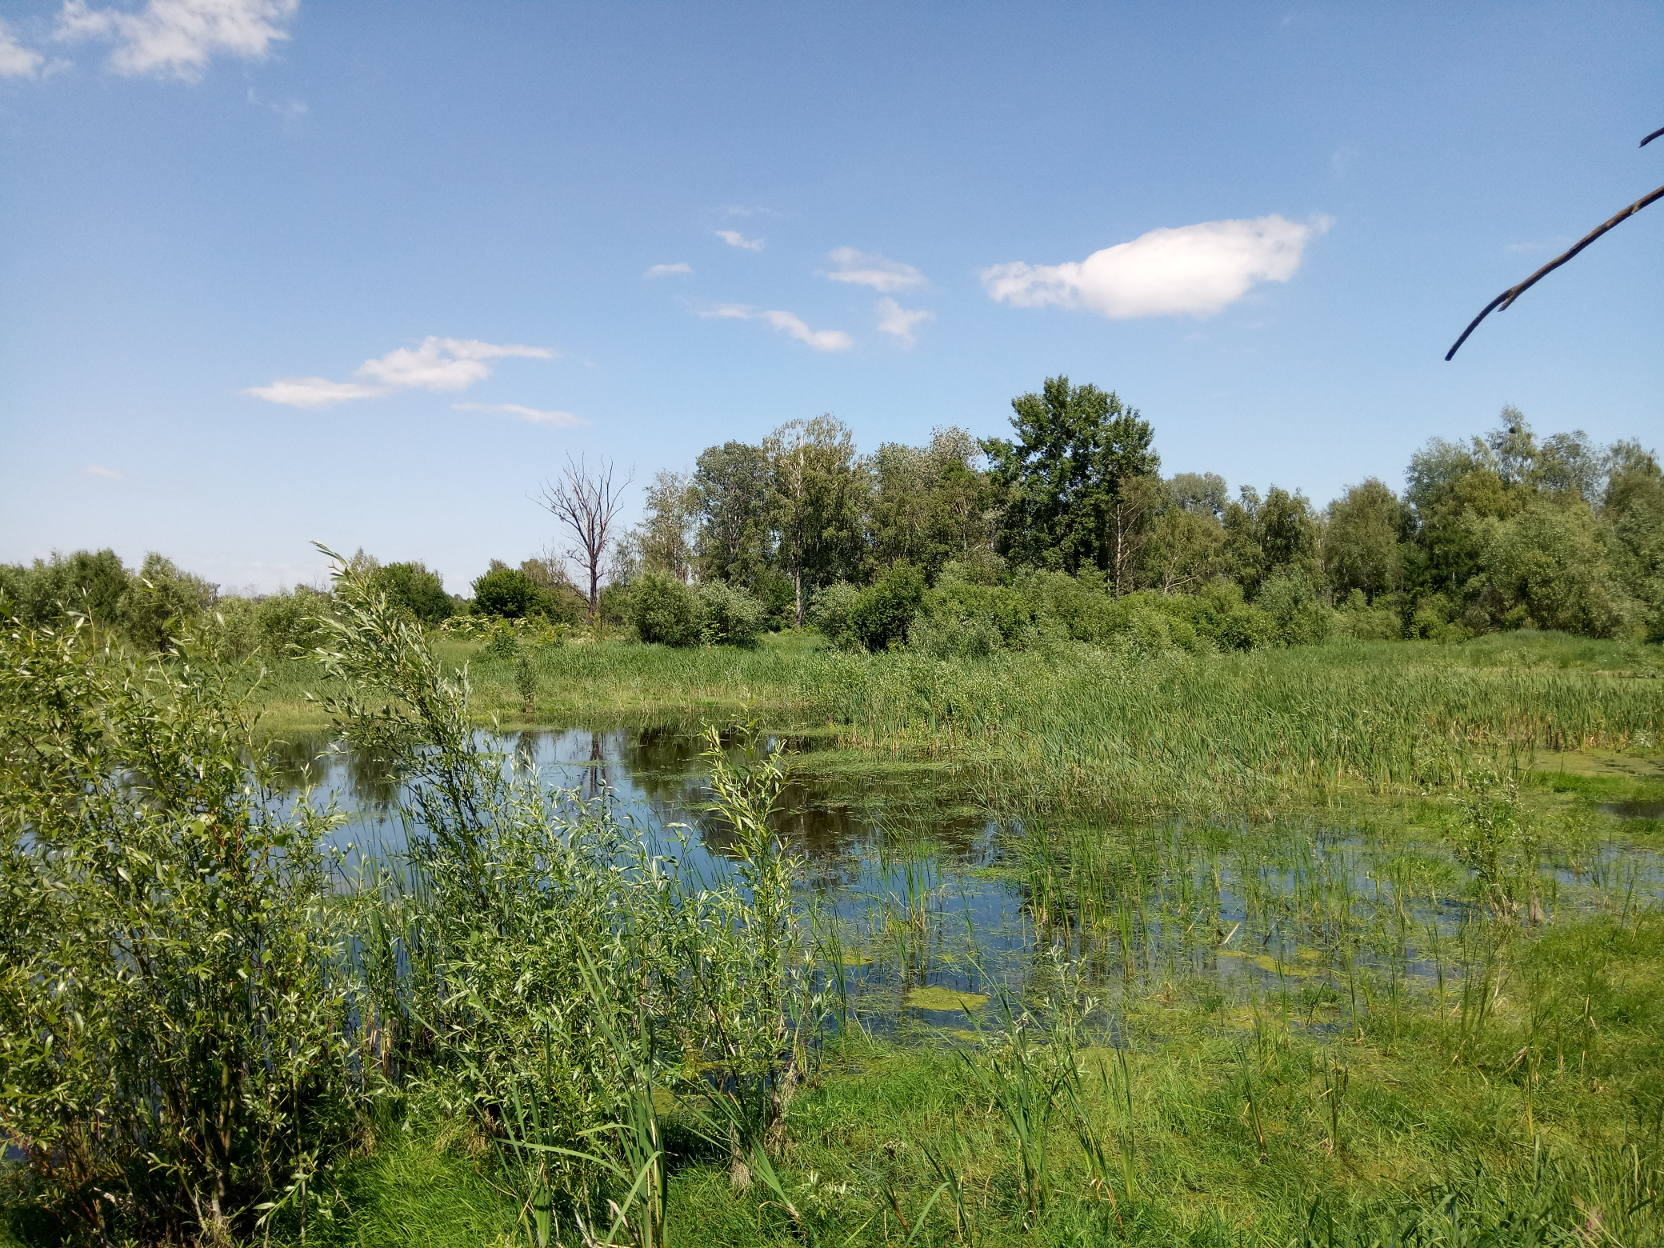
\includegraphics[width=\linewidth]{chast-gorodki/kolpit/kov01-r.jpg}

\textit{2018, южная часть Ковпыта.}
\end{center}

В 19 веке, западнее Ковпыта, по хребту вытянутого с севера на юг холма, продолжался сосняк, затем его сменяли кусты и невысокие деревца, и там-то, параллельно Ковпыту раскинулось другое, даже большее болото. Между ним и Ковпытом – высокая гора, в одном месте\footnote{50°30'47"N, 30°40'5"E} понижающаяся. Там между болотами, из одного в другое, был канал.

\begin{center}
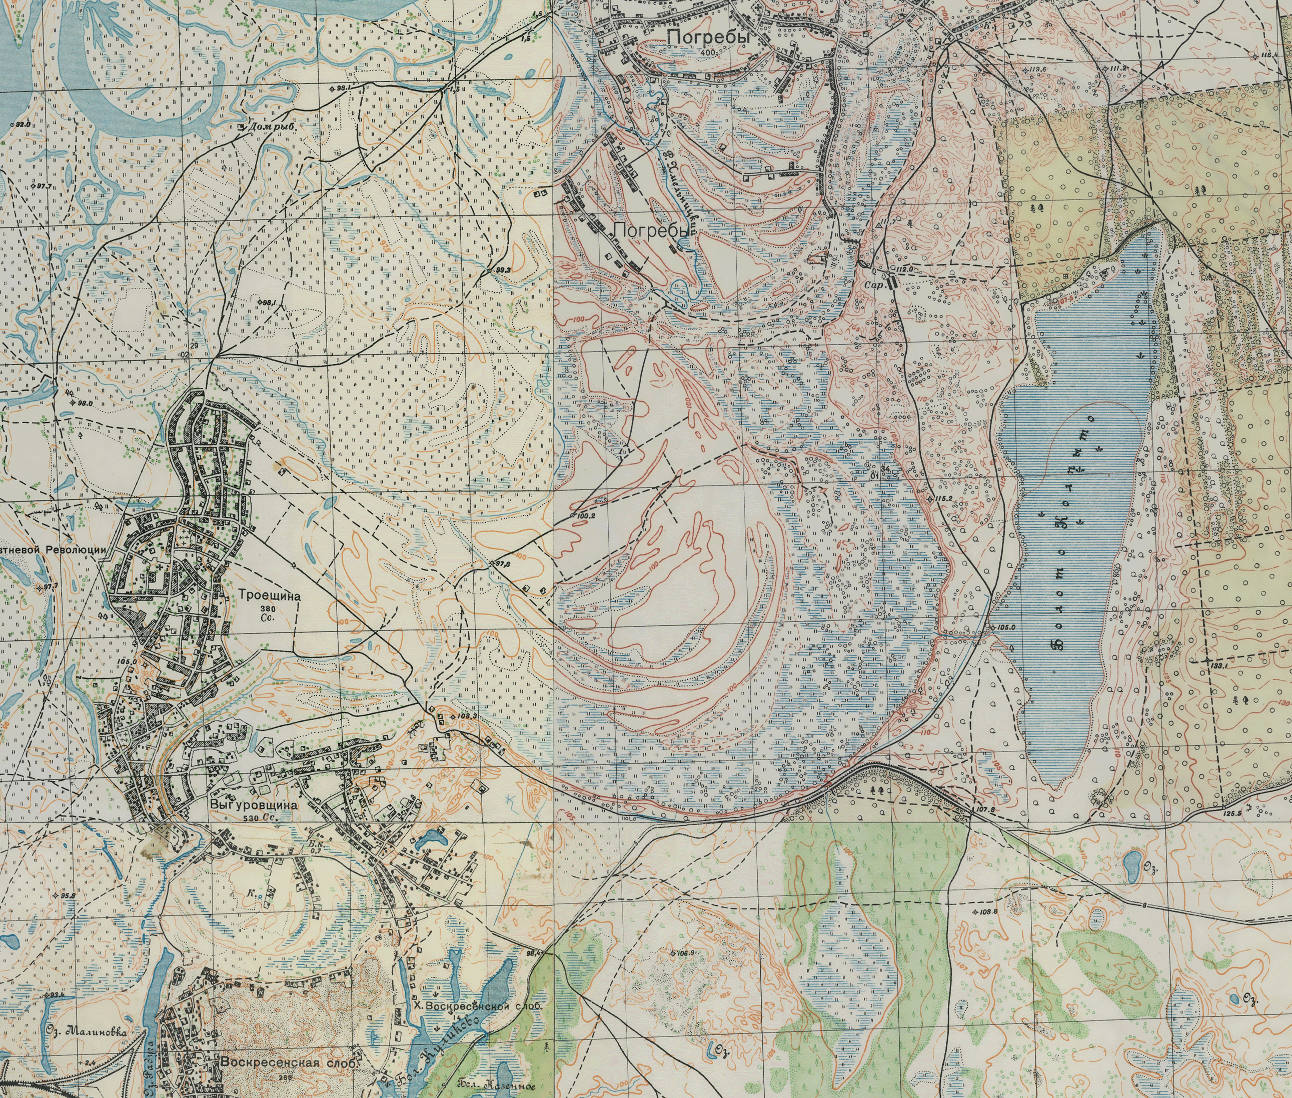
\includegraphics[width=\linewidth]{chast-gorodki/kolpit/rkka-kolp.jpg}

\textit{Кусок плана РККА 1930-х.}
\end{center}

Второе это болото не удостаивалось подписи на картах, однако поглядите на карту РККА 1930-х. Вот оно, слева от Ковпыта. Что напоминает? Поворот огромной реки.

Некогда это было древнее русло Десны, поворачивающее тут к Днепру. Где же остальное русло? А есть – та полоса болот, что тянулась вдоль восточного берега Десны на десятки километров, между нею и бором.

Десна отступила на запад, а в старом русле образовались болота. Между современным руслом и давним находятся такие близкие к Киеву селения, как Погребы, Зазимье, Пуховка, Летки. По карте видно – старинное русло выруливает ниже Погребов к Днепру в направлении Выгуровщины с Троещиной. Прудок выглядит продолжением изгиба русла.

Безымянное болото в повороте своем превратили в крупнейшее озеро Киева – Алмазное. Отживает прежнее его название, Торфы. Там добывали торф. А рядом выращивали кукурузу и горох.

Когда строили жилмассив Троещину, понадобился песок. Торфы превратились в чудовищный карьер – 3 километра длиной, более 600 метров шириной, 35 глубиной. Такие размеры сохраняет и нынешнее озеро. Карьер наполнился водой и стал Алмазным озером. А как видим по карте РККА, в середине 20 века Ковпыт довольно глубок, а место Алмазного – хотя и болото, но смешано с заливными лугами.

Если вы не гуляли в окрестностях, советую поглядеть мой фильм «Шелест Быковнянского леса», где всё показано – и Большая поляна, и Алмазное озеро, которое я объехал кругом на велосипеде.

Да расскажу словами, добавив кое-что сверх. Будем идти от Большой Поляны. Так ее называют жители Лесного массива. На картах это место иногда обозначают как «урочище Куричево». В давних земельных документах, которые мы будем разбирать позже, упоминается болото Куричево, однако насколько верно сопоставление Большой Поляны и этого старинного болота? По некоторым соображениям, Куричево – это нынешнее Алмазное озеро. Хотя на месте Большой Поляны еще в 1930-х в самом деле было большое болото, окруженное хвойным лесом. Западный берег того болота сейчас возвышается круто, местами метров на шесть-семь, и переходит в довольно высокую местность, слывущую на картах как Сухие Горы. На песке там растут сосны.

Поляна прячется в лесу за Лесным кладбищем и южнее. Привольный луг с густой высокой травой, пахнет здорово, гудят пчелы. К востоку шумит березняк. У березы листья маленькие, жесткие, треплются на ветру язычками. Там в бело-зеленой глубине есть озеро со спокойной водой. Ему по меньшей мере сотня лет.

\begin{center}
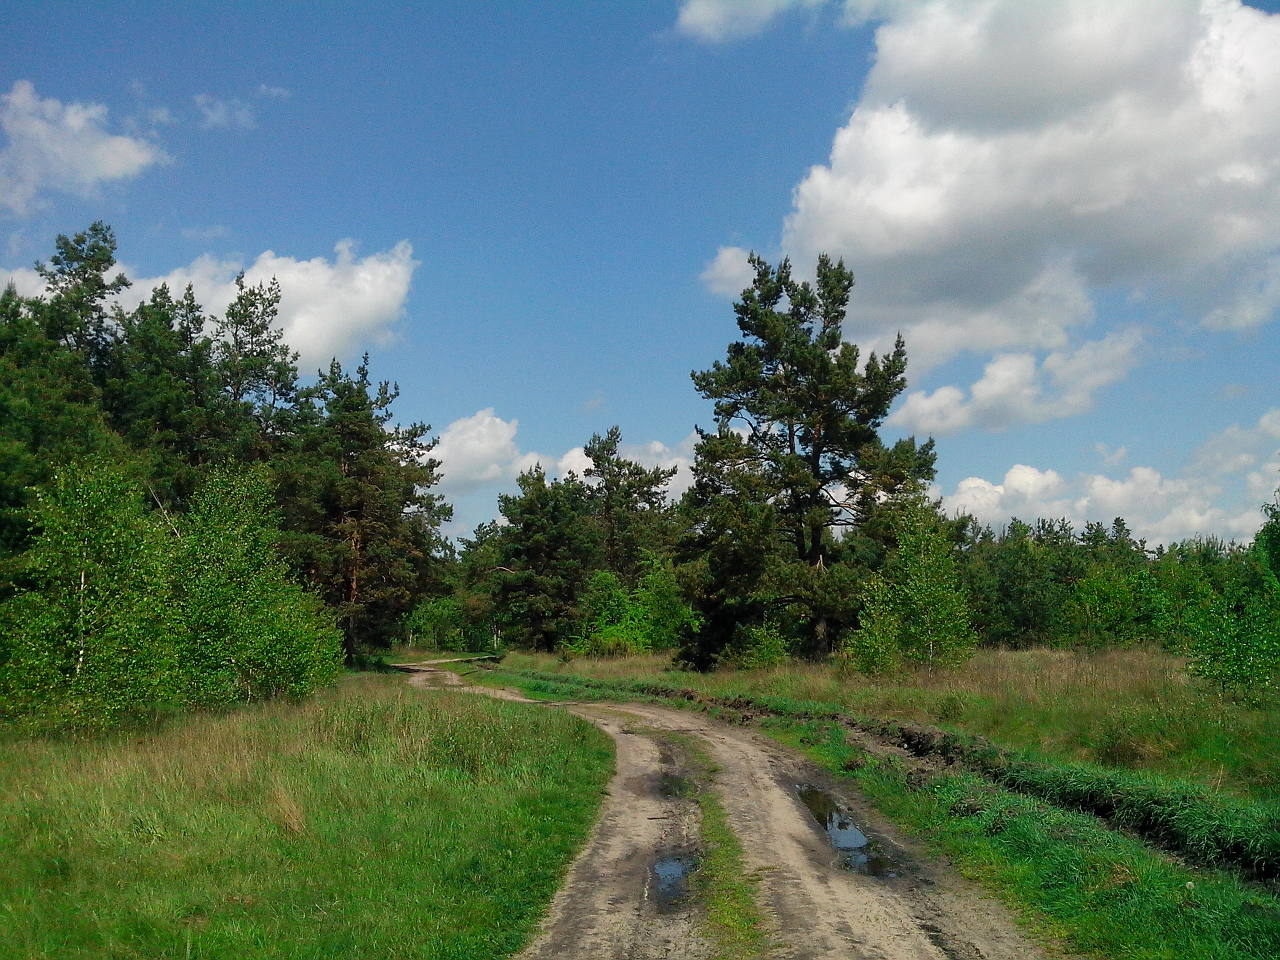
\includegraphics[width=\linewidth]{chast-gorodki/kolpit/s_IMG_20140513_115717.jpg}

\textit{Север Большой поляны, май 2014.}
\end{center}

Вообще в этих краях раньше, при царе, была окраина артиллерийского полигон, условно говоря от метро «Дарница» до «Лесной» и от этой линии на северо-восток (жилмассивы вдоль Малышко и Юности, Бойченко, Водопарк). Поныне в лесу за Жукова есть образованные взрывами котлованы, уже затянувшиеся землей, сглаженные. А однажды я шел по лесу, гляжу – лежит снаряд. Целехонький и чужеродный. Может, выкопал кто и бросил, далеко тащить такую тяжесть.

К западу от Большой Поляны – лиственный лес, местами переходящий в болото, и полоса корявого березняка в низине, ограниченной могучими дюнами Сухих Гор.

Наивно думать, что Левый берег сплошь плоский! Южная сторона Лесного кладбища примыкает к этим холмам и лежит вдоль склона горы. На велике можно долго ехать мимо кладбищенской ограды, не крутя педали. Наоборот, приходится даже тормозить.
 
Мы, двигаясь на север, проходим Большую поляну, и после небольшого лесочка снова цвиринькает кузнечиками луг, а вдали видно сосновый лес. Еще в начале 21 века на месте поля тоже росли сосны, но потом огромный их участок вырубили, а пни выкорчевали. За левой обочиной дороги прячется мелиоративный канальчик, иногда по нему даже что-то сочится. Грунтовка начинает петлять, в ямах стоит мутная вода. После дождя тут невозможно пройти.

Вскоре дорога оказывается на пригорке и упирается в другую – остатки давнего шляха. Между ним и Алмазным – полоса деревьев, за которыми светлеет пространство – так всегда бывает, когда впереди вода. О ней пока только догадываешься по запаху. И мы идем вперед, по тропке через чашу, и оказываемся на косогоре, затем переходящем в обрывистый берег, точно такой, как бывает на Десне, с соснами и ласточкиными норами. А под ним лежит Алмазное озеро.

Вот оно на снимках 2014 года:
\vspace*{\fill}
\begin{center}
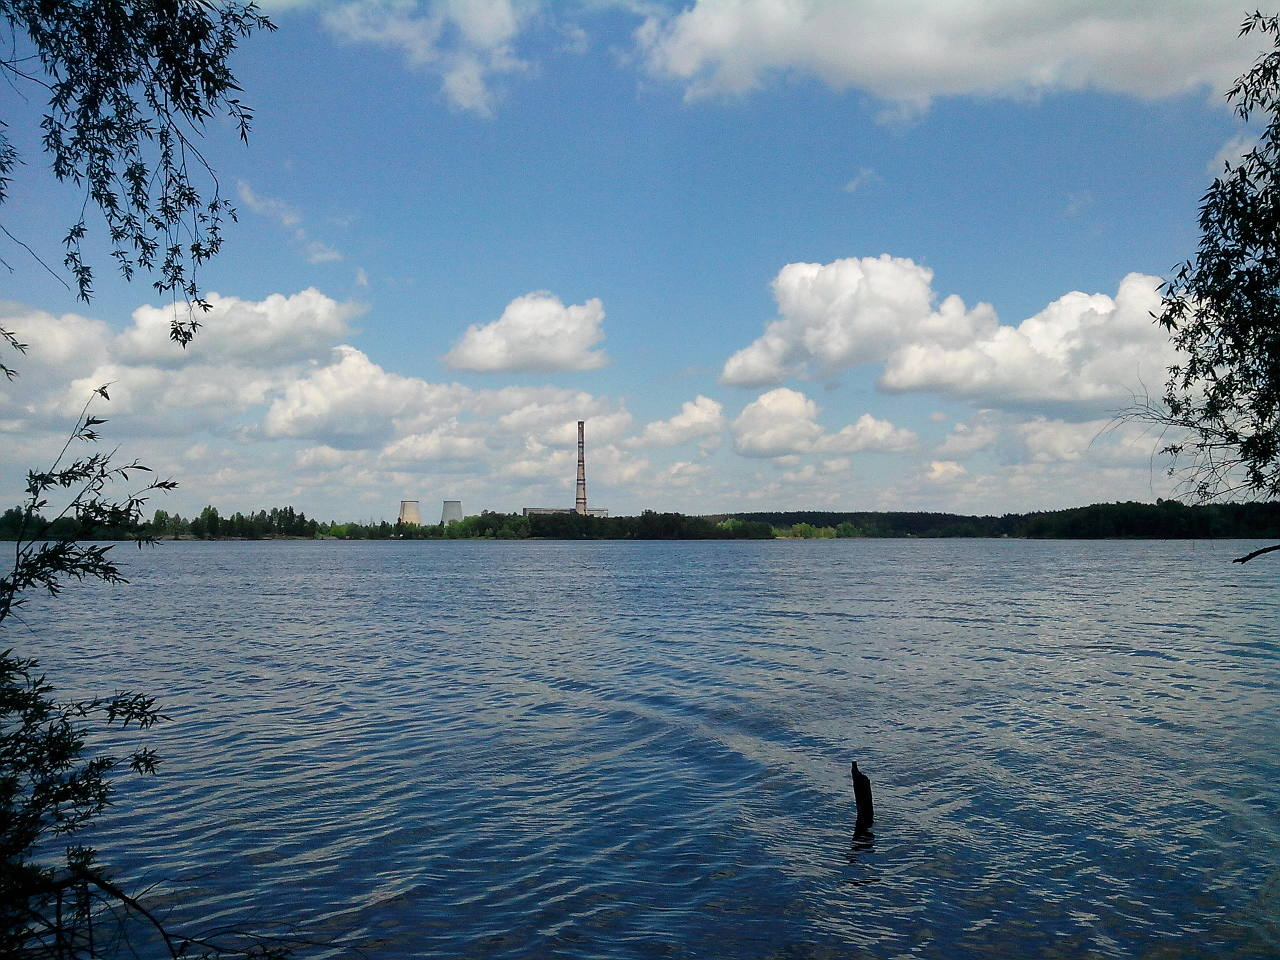
\includegraphics[width=\linewidth]{chast-gorodki/kolpit/s_IMG_20140513_124640.jpg}
\end{center}
\vspace*{\fill}
\newpage

\begin{center}
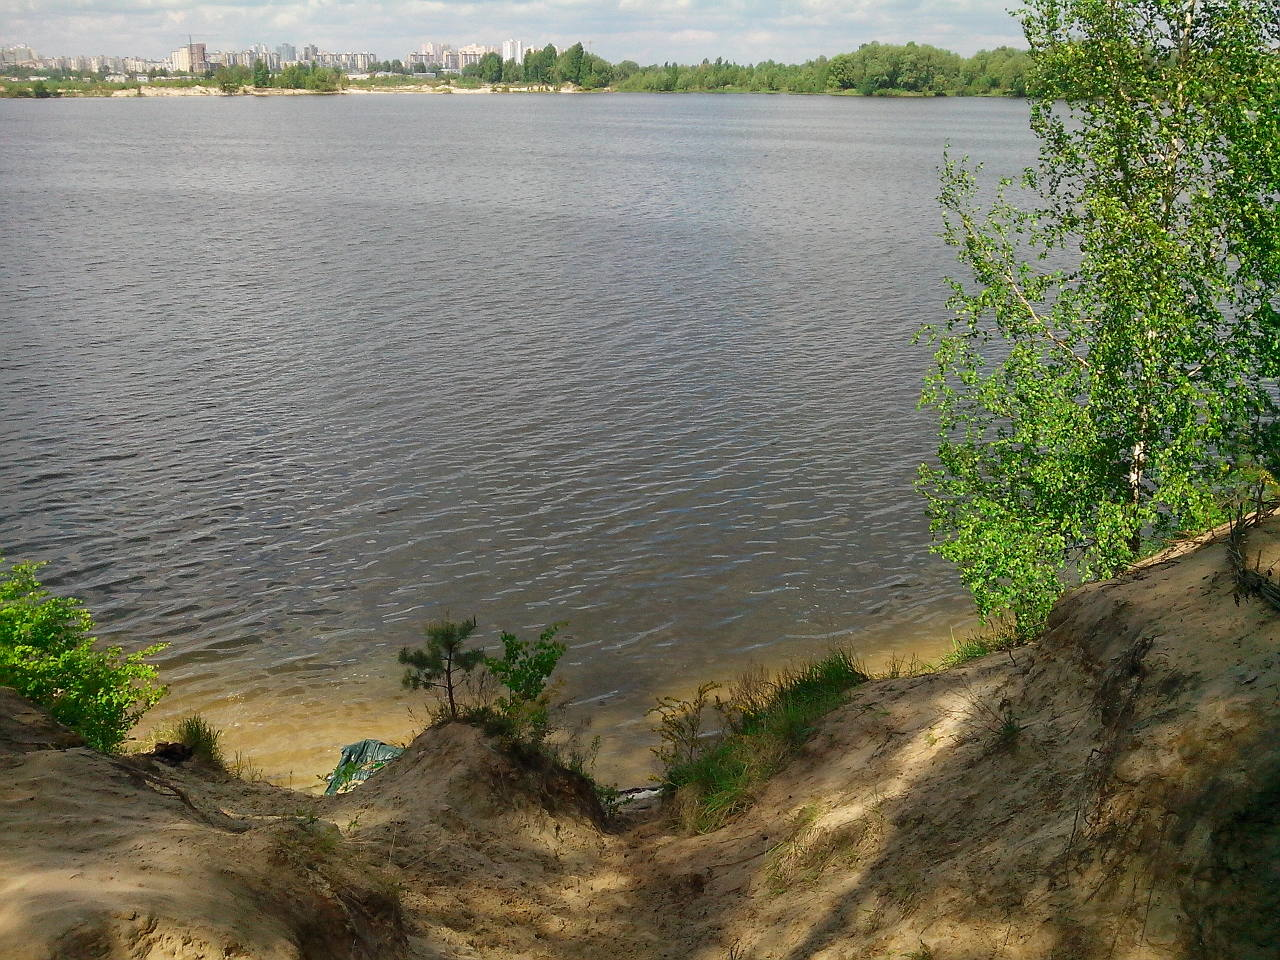
\includegraphics[width=\linewidth]{chast-gorodki/kolpit/s_IMG_20140513_123046.jpg}
\end{center}

Далеко, на противоположном западном берегу – промзона и песчаный карьер. Нет, монетный двор\footnote{Бывший завод «Алмаз». Остановка около него по 2016 год так и называется – «завод Алмаз». Потому и озеро Алмазное.} чуть дальше, за улицей Пуховской, идущей параллельно Алмазному среди заболоченных лугов. Улица даже не улица, а заасфальтированная дорога, ведущая к ТЭЦ-6 и Погребам. ТЭЦ-6 тоже стоит на горе, ведь склон, составляющий южную и восточную часть берега Алмазного озера, продолжается и к северу от него, возвышаясь над еще заболоченным участком древнего русла Десны.

Склон будто обнимает это русло рукой. Над дорогой вдоль северной оконечности Алмазного, среди сосен – стихийное кладбище домашних животных, а восточнее уже официальное, недостроенное. Поминальная ротонда, административное здание, валяются бетонные блоки, вход зарастает бурьяном.

Восточнее кладбища – три отстойника ТЭЦ-6, ее технические пруды с известковым шлаком. В заводненном отстойнике живут странные рыбы, а земля вокруг рыжая.

От прудов, через полотно железнодорожных подъездных путей ТЭЦ – недостроенный асфальтный завод. Бетонные каркасы зданий среди песка и кустов. Там раньше играли в пейнтбол. Понемногу вырастают молодые сосенки. Это у южной стороны ТЭЦ-6.

А у северо-восточной, в лесочке\footnote{50°32'13"N 30°40'38"E} – кладбище человеческое, с могилами от времен Великой Отечественной и по наши дни. Оно лежало на северном берегу Ковпыта. Карта РККА начала 1930-х годов показывает в том месте некое строение с оградой. Возможно там и находился известный по плану Шуберта «двор стражника». Кладбище же по плану РККА – в полутора сотнях метров на восток\footnote{50°32'13.7"N 30°40'44.0"E} от современного.

Северная же часть Алмазного озера – продолжение южного конца существующего поныне болота (параллельного Ковпыту, на запад, и отделенного от него горой), части той давней полосы болот, в которой я предполагаю прежнее русло Десны.

Сверху озеро и болото выглядят единым полумесяцем, щербиной на запад. Так было и когда по Выгуровщине протекал Прудок, только вместо прозрачной желтизны Алмазного озера зеленело болото. Но воды хватало. И куда она девалась? Вытекала ручьем, что в пределах Выгуровщины люди называли – Прудок.

Сейчас вода Алмазного из западной части озера попадает в коллектор, что проходит потом под проспектом Ватутина.
